\documentclass[11pt]{article}
\usepackage{tikz}
\usetikzlibrary{trees}
\usetikzlibrary{positioning}
\tikzset{main node/.style={shape=rectangle,
    draw, align=center,
    top color=blue!10, bottom color=blue!10}}
\usepackage{amsfonts}
\usepackage{amsmath}
\usepackage{verbatim}
\setlength\parindent{0pt}
\begin{document}
\title{Force-Based Physics Simulator}
\author{Zachary Kieda (zkieda@andrew.cmu.edu)}
\date{\today}
\maketitle

\begin{section}{Introduction}
For this project, we will build a force-based physics simulator. Typically, physics simulators use a posteriori (discrete) methods of detecting collisions and simulation. In these simulators, the scene applies all forces to objects, calculates the new accelerations, velocities, and the new positions of the objects. Then, the simulator will check if any two objects have collided, and will compensate accordingly. \\

A limitation of this method is that it can be inaccurate and miss collision detection of fast moving objects. A second limitation is that it gives only low-level information about the collisions and mechanics of the scene. This makes discrete simulators tough to use in robotic applications, but makes it suitable for simulating a physics phenomenon.\\

Our system will be an a priori (continuous) event-based simulation. In contrast to a posteriori systems, ours will find the next event that will occur and move the scene up till that point and continue. During the simulation, a user will have access to higher-level information -- e.g. the exact time that an object should collide in the future, the next event that should occur, and the force, velocity, and position of the future collision.\\

We define a client as a user of our simulation. The client has the responsibility of setting up the scene and its properties. While the simulation is running, the client can choose to apply forces to dynamic objects in the scene. The client also has the option of viewing what the modifications would do, and backtrack if necessary. This makes our simulator ideal for robotic simulation, and for creating novel algorithms for interacting with an environment.\\
\end{section}


\begin{section}{Client API}
To use the library, the client must define a "Problem" that will be solved by the simulator. The client generates a problem from a world, simulation, and evaluator. The simulation defines the the properties that we should use during the simulation, the evaluator defines the client's method for applying forces to achieve their goal. There are default simulation classes available to the client which allow them to simulate in two and three dimensions, and with additional options like the integration technique. \\

The client API consists of two main parts, the world and the evaluator. Our simulator is written in python, and a python-based language would be useful to utilize the library.

\begin{subsection}{The World API}

We define many defaults objects that the client can simulate, but we also ensure that the library is extensible in case if the client wanted to simulate something that is not available inside of our library. We believe that our library provides primitives useful for most simulation tasks. We break down the general object hierarchy in Figure 1. Lines are drawn down towards subclasses. Since this is python, a class may have multiple superclasses (lol).\\

\begin{center}
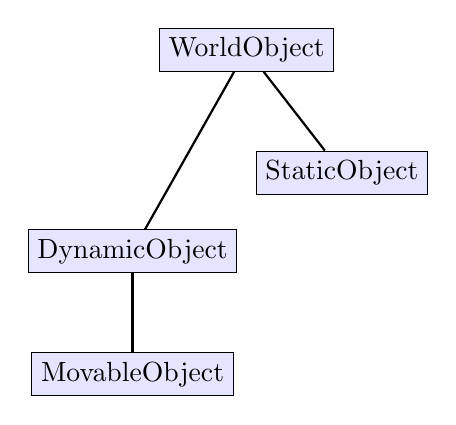
\begin{tikzpicture}
    \node[main node] (1) {WorldObject};
%    \node[main node] (2) [right = 2.5cm  of 1] {Tri};
%    \node[main node] (3) [right = 1.75cm  of 1] {Particle};
%    \node[main node] (4) [right = 1.75cm  of 3] {Mesh};


	\node[main node] (5) [below right = 1cm and -1cm of 1] {StaticObject};
	\node[main node] (6) [below left = 2cm and -1cm of 1] {DynamicObject};
	
	\node[main node] (7) [below = 1cm of 6] {MovableObject};
	

%	\node[main node] (11) [below = 1cm of 4] {StaticMesh};	
	
%	\node[main node] (8) [below = 3.0cm of 3] {DynamicParticle};
%	\node[main node] (9) [below = 1.5cm of 11] {DynamicMesh};
	

    \path[draw,thick]
    (1) edge node {} (5)
    (1) edge node {} (6)
    (6) edge node {} (7)
    
%    (3) edge node {} (8)
%    (4) edge node {} (9)
    
 %   (6) edge node {} (8)
 %   (6) edge node {} (9)
    ;
\end{tikzpicture}\\[0.5cm]
\textbf{Figure 1.} The World's General Object Hierarchy
\end{center}
In Fig. 1 we can see the general layout for the objects that the client can use. At the end of the day, the client can add any WorldObject to set up the scene, but the other classes provide additional functionality as well. The DynamicObject are objects that can move around in the scene after initialization has occurred, and external forces are applied to the objects. A StaticObject, on the other hand, do not move, and only provide boundaries for collisions. A MovableObject is a type of DynamicObject such that the client can modify the forces that are effecting the object while the simulation is running. All active DynamicObjects are presented to the client during the simulators evaluation, while DynamicObjects that are not MovableObjects are not. \\

From here, we present two distinct types of objects that the client may add in. Figure 2 shows the class hierarchy used for particles, and Figure 3 shows the class hierarchy for Meshes. \\

\begin{center}
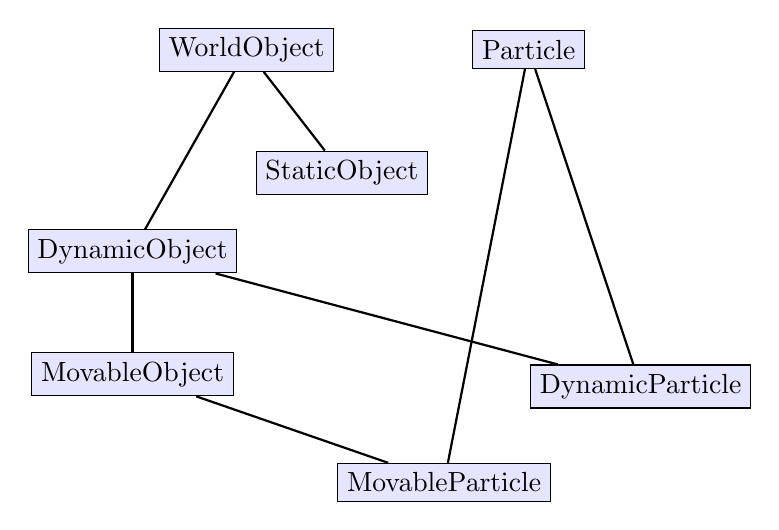
\begin{tikzpicture}
    \node[main node] (1) {WorldObject};
%    \node[main node] (2) [right = 2.5cm  of 1] {Tri};
    \node[main node] (3) [right = 1.75cm  of 1] {Particle};
%    \node[main node] (4) [right = 1.75cm  of 3] {Mesh};


	\node[main node] (5) [below right = 1cm and -1cm of 1] {StaticObject};
	\node[main node] (6) [below left = 2cm and -1cm of 1] {DynamicObject};
	
	\node[main node] (7) [below = 1cm of 6] {MovableObject};
	

%	\node[main node] (11) [below = 1cm of 4] {StaticMesh};	
	
	\node[main node] (8) [below right = 3.75cm and -.70cm of 3 ] {DynamicParticle};
	\node[main node] (9) [below left = 5cm and -1.0cm of 3 ] {MovableParticle};
%	\node[main node] (9) [below = 1.5cm of 11] {DynamicMesh};
	

    \path[draw,thick]
    (1) edge node {} (5)
    (1) edge node {} (6)
    (6) edge node {} (7)
    
    (3) edge node {} (8)
    (3) edge node {} (9)
    
    (6) edge node {} (8)
    (7) edge node {} (9)
    ;
\end{tikzpicture}\\[0.5cm]
\textbf{Figure 2.} The World's Object Hierarchy for Particles
\end{center}

Note that we do not have static particles. However, we are leveraging the multiple inheritance to allow a particle to be dynamic or movable by using the superclass as a mixin.\\

Finally, in Figure 3 we show the class hierarchy for Meshes. Note that we have StaticMeshes, DynamicMeshes, and MovableMeshes.

\begin{center}
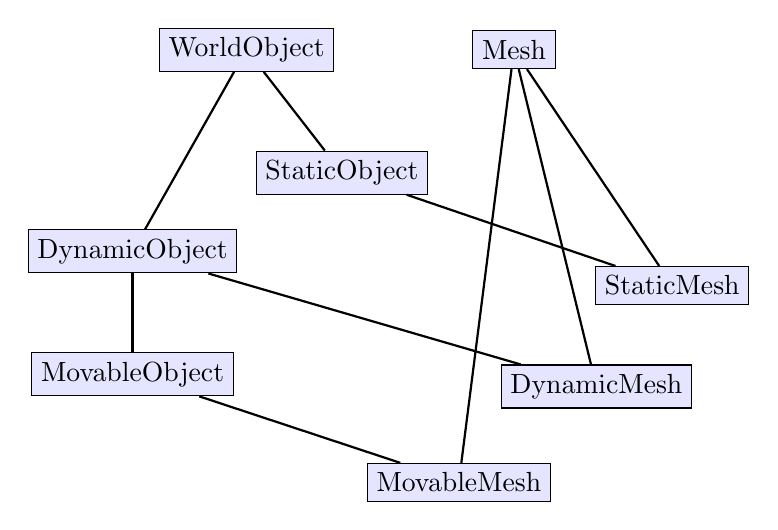
\begin{tikzpicture}
    \node[main node] (1) {WorldObject};
%    \node[main node] (2) [right = 2.5cm  of 1] {Tri};
    \node[main node] (3) [right = 1.75cm  of 1] {Mesh};
%    \node[main node] (4) [right = 1.75cm  of 3] {Mesh};


	\node[main node] (5) [below right = 1cm and -1cm of 1] {StaticObject};
	\node[main node] (6) [below left = 2cm and -1cm of 1] {DynamicObject};
	
	\node[main node] (7) [below = 1cm of 6] {MovableObject};
	

%	\node[main node] (11) [below = 1cm of 4] {StaticMesh};	
	
	\node[main node] (8) [below right = 3.75cm and -.70cm of 3 ] {DynamicMesh};
	\node[main node] (9) [below left = 5cm and -1.0cm of 3 ] {MovableMesh};
	\node[main node] (10) [below right = 2.5cm and 0.5cm of 3 ] {StaticMesh};
%	\node[main node] (9) [below = 1.5cm of 11] {DynamicMesh};
	

    \path[draw,thick]
    (1) edge node {} (5)
    (1) edge node {} (6)
    (6) edge node {} (7)
    
    (3) edge node {} (8)
    (3) edge node {} (9)
    (3) edge node {} (10)
    
    (6) edge node {} (8)
    (7) edge node {} (9)
    (5) edge node {} (10)
    
    ;
\end{tikzpicture}\\[0.5cm]
\textbf{Figure 2.} The World's Object Hierarchy for Meshes
\end{center}
StaticMeshes simply are world geometry. We can simulate walls in two dimensions through multiple two dimensional static meshes. For DynamicMeshes and MovableMeshes we ensure that force will be applied to the object as a whole. \\

\emph{Note} We're currently unsure how we should deal with DynamicMeshes with respect to the masses that they may have. Typically, for a solid, we would want to have the mass evenly distributed throughout the hull. If we were to assign weight to the surface, this would not produce the same result. Therefore, we may place the restriction that all DynamicMeshes must be solid and closed. 

\end{subsection}

\begin{subsection}{The Evaluator API}
\emph{Note} This section may change in the future, as this API is not yet complete.\\

The purpose of the evaluator is to give as much freedom to the client. The purpose of our project is to not provide them with an automatic solver for an arbitrary problem. However, we support helper functions that can help clients keep track of their goal, as well as a basic solver for movable particles.\\

In the API, we provide a target-tracking method. The client defines a destination transformation that should be applied to each of the MovableObjects, and we bundle this data structure as $\emph{Progress} = (\emph{MovableObject} \times \emph{DestT}\times\emph{FinalV})$, where $DestT$ is the destination transform matrix. We also provide a basic evaluator for the progress, which finds the difference from the current transformation matrix to the final transformation matrix. The matrix should only perform positional movement and rotational changes. $FinalV$ represents a 3-dimensional or 2-dimensional target velocity vector that the MovableObject should eventually have. Again, we provide basic methods that track this change, but the method can be overridden by the client.\\

In the previous simulator iteration, there was a Target coupled to each particle. This has been decoupled, as the final targeting system used should be determined by the client. \\

\textbf{Controlling MovableObjects}\\
The client passes in an Evaluator to control the MovableObjects. 
\begin{verbatim}
Problem
    + getHandle() : Handle
    + simulate(forceInfo : array, doPlot : Boolean)
    ...
State
    + getTime()
    + getWorld()
    ... (some helper functions for high level functionality)
Handle
    + getOtherSteps() : Handle list
    + currentState() : State
    + stepBack() : Handle
    + stepForward() : Handle
      /* Steps till next event/timestep. 
       * Will tell client if it's an event or
       * if we stopped at a timestep.
       */
    + stepDt(dt : double) : State
      /* Steps forward by dt */
    + stepBackTill(evt : event) : State
    + stepForwardTill(evt : event) : State
    + applyActiveForce(object : MovableObject, 
        force : np.array, dt : phase) : (Handle, id : int)
    + applyActiveForces(object : MovableObject, 
        forceInfo : (np.array, phase) list) : (Handle,  ids : int list)
      /* Applies multiple forces over time */
    + removeActiveForce(id : int) : Handle
      /* manually remove force */
    + getActiveForceInfo(id : int) : (object, force, dt)
    + getActiveForces() : int list
    + getActiveForcesByObject(object) : int list
Evaluator
    + run(handle : Handle) : () 
      /* Passes a handle to the evaluator, which the evaluator then runs. */
\end{verbatim}
 %  + mark() : id : int
  %  + loadMark(id : int)
   % + removeMark(id : int)
Note that the sole purpose of the Evaluator is to accept a handle, then to run the simulation till its completion. The evaluator will contain all of the logic for running the simulation. The client adds forces to the current simulation, choosing the force strength, position, and object that it's acting upon. The client defines a \emph{phase} that the force should act over, such that we define the interval, starting time, and duration that the force should run for. The client has the choice of adding the force, moving the system forward and testing the result, then possibly modifying or removing the force and going back to a previous state. The client can also define many forces that should be applied over different phases.\\

The functions \verb|stepBackTill| and \verb|stepForwardTill| allow the client to define functions that will cause the simulator to step till some criteria is satisfied. For example, we could go to previous states until we were at the beginning. Or, we could continue stepping forward till a particle collides with a certain surface.\\

The function \verb|getOtherSteps| allows the client to see the other steps that they have taken from this exact time. Note that this will also modify the list of active forces. This allows backtracking easy for the user. Then, using the Handle is like a tree traversal exploring  possibilities. We hope to add in a method that will permit a client to garbage collect unused or dead branches. This might be possible with a mark system, where the client explicitly marks the trees that they may want to revisit, and rewind to the previous mark if necessary. It would also be nice to provide a function that would allow a client to compare their handle to another, giving information about the forces that were or were not applied in the different versions, as well as the important differences in their outcomes.\\

\end{subsection}
\end{section}
\begin{section}{Events}
In this section, we will discuss and enumerate the event types that can occur in the simulator. We will briefly overview the (currently implemented) events in two dimensions, then we will discuss the newly implemented events in three dimensions.

\begin{subsection}{2D Events}

\textbf{Currently implemented}\\
\begin{itemize}
\item Particle Collision event: Occurs when a particle hits a manifold
\item Particle Zero Velocity event: Occurs when a particle reaches zero velocity, typically from frictional forces. 
\item Particle Boundary crossing event: Occurs when a particle crosses a boundary on a mesh. This occurs when a particle leaves a boundary, or when a particle moves from one boundary from another.
\end{itemize}

\textbf{Not yet implemented}\\
\begin{itemize}
\item Mesh Collision event: occurs when a dynamic mesh hits another mesh. We enumerate proposed possibilities below
\begin{itemize}
\item Mesh point on mesh point
\item Mesh point on mesh edge
\item Mesh edge on mesh edge
\end{itemize}
\item Mesh Zero Velocity event: occurs when a mesh reaches zero velocity.
\item Mesh Boundary Crossing event: Deals with boundary crossing with respect to dynamic meshes. 
\end{itemize}

\end{subsection}
\begin{subsection}{3D Events}

Note that the particle events will be the same in three dimensions as it was in two dimensions. We merely extend collisions and boundary crossings from a line boundary to a plane boundary. We will not have events between particles, as discussed previously. \\

To help define different events, we define a meta-classification (the event type), and a sub-classification (the event class).\\

We have three event types, a zero-velocity event, a collision event, and a boundary crossing event. Event classes only differ from one to three dimensions.\\

\textbf{Mesh on Mesh classes}\\
All of these classes occur both for both collision events and boundary crossing events.
\begin{itemize}
\item Mesh vertex on mesh vertex
\item Mesh vertex on mesh edge
\item Mesh edge on mesh edge
\item Mesh vertex on mesh plane
\item Mesh edge on mesh plane
\item Mesh plane on mesh plane
\end{itemize}

\end{subsection}
\end{section}
\begin{section}{Implementation}

\begin{subsection}{Currently Implemented}
\begin{itemize}
\item Refactor the code-base for WorldObjects, DynamicObjects, etc.
\begin{itemize}
\item Refactored particle system
\item Have framework for meshes, but no collisions and movement for dynamic meshes or movable meshes 
\end{itemize}
\item Refactored codebase to allow three-dimensional characteristics. 
\item Changed code to use StaticMeshes instead of boundaries, using each face of the mesh as a boundary. 
\item Changed code such that the target is decoupled from the actual object, which we track within the evaluator.
\item Added library for the Evaluator and Handle. Partially implemented.
\begin{itemize}
\item Complete : stepBack/Forward, stepDt
\item Complete : applyActiveForce[s], removeActiveForce
\item Complete : getOtherSteps, getActiveForce[s], getActiveForcesByObject, getActiveForceInfo
\item Todo : stepBackTill, stepForwardTill
\end{itemize}
\item Framework for mesh events are completed in two and three dimensions (for boundary crossing, surface events, etc). 
\end{itemize}
\end{subsection}
\begin{subsection}{Todo}
\begin{itemize}
\item Complete work on meshes, both in two and three dimensions.
\item Formalize rules for mesh events, write them in this paper.
\item Be able to check if dynamicmeshes are closed. Find the center of mass of a closed mesh.
\item Be able to calculate acceleration, velocity, and position changes in mesh given the forces applied and the current state.
\item Supply client with API for tracking their progress with respect to the current state. 
\item Supply client with API for high level information about the state (also define what API is needed).
\begin{itemize}
\item Possible : find phases that will be able to make simple event occur given current state, like having a movable particle collide with a mesh, or to cross a surface boundary. 
\item Possible : Give information ``this particle is currently on this collision manifold", or a list of active events that they can filter. 
\item Test cases.
\item Visualization in three dimensions
\end{itemize}
\end{itemize}
\end{subsection}
% solids need inertia
\end{section}
\end{document}